\documentclass[12pt]{article}

\usepackage{sbc-template}
\usepackage{graphicx,url}
\usepackage[utf8]{inputenc}
\usepackage{amsmath, amssymb}
\usepackage{booktabs}
\usepackage{subfigure}
\usepackage[
    backend=biber,natbib,
    style=authoryear
]{biblatex}

\addbibresource{references.bib}

\newcommand{\SubItem}[1]{
    {\setlength\itemindent{15pt} \item[-] #1}
}
     
\sloppy

\title{Modelagem e Previsão de Tráfego de Rede:\\ Uma Abordagem para ISP's}

\author{Murilo A. Chianfa\inst{1}, Bruno B. Zarpelão\inst{1}, Sylvio B. Junior\inst{2} }


\address{Departamento de Computação -- Universidade Estadual de Londrina
  (UEL)
  \nextinstitute
  Departamento de Engenharia Eletrônica e Arquitetura -- Universidade de Trieste (UNITS)
  \email{\{murilo.chianfa,brunozarpelao\}@uel.br, sylvio.barbonjunior@units.it}
}

\begin{document} 

\maketitle

\begin{abstract}
  This study develops a method for network administrators to conduct extensive tests on traffic data using various time series forecasting models. Three algorithms were selected: SARIMAX, Prophet, and LSTM. The portal assists in selecting the best model, optimizing hyperparameters, and evaluating the trade-off between time and prediction efficiency.
\end{abstract}
     
\begin{resumo} 
  Este estudo desenvolve um método para que administradores de rede possam realizar testes extensivos em dados de tráfego utilizando diversos modelos de previsão de séries temporais. Três algoritmos foram selecionados: SARIMAX, Prophet e LSTM. O portal auxilia na escolha do melhor modelo, na otimização de hiperparâmetros e na avaliação do tempo versus eficiência das previsões.
\end{resumo}


\section{Introdução}

Atualmente, com o advento de novas tecnologias no setor de telecomunicações, como Internet das Coisas (IoT),  WiFi-7 e XGS-PON, estamos enfrentando um grande aumento no volume de tráfego de rede produzido como nunca antes visto [\cite{fleischer_using_2017}]. Provedores de Serviço de Internet (ISPs) tentam implementar técnicas de monitoramento e análise de dados para tentar otimizar o fluxo de trabalho dessas redes, mas técnicas tradicionais têm se mostrado ineficazes para este trabalho.

Previsão de tráfego de rede desempenha um papel fundamental no avanço das redes de computadores, áreas como gerenciamento, design, alocação de recursos, engenharia de tráfego e detecção de anomalias [\cite{troia_identification_2017}]. Duas principais categorias de predição são atualmente empregadas, \textit{long-term} e \textit{short-term}. \textit{Long-term} atualmente é mais utilizada para planejamento futuro de capacidade e recursos necessários, já \textit{Short-term} sendo empregada para melhorar a qualidade dos serviços como Qualidade de Serviço (QoS) e alocação dinâmica de recursos [\cite{andreoletti_network_2019}].

\subsection{Objetivos da pesquisa}

O principal foco desta pesquisa é desenvolver um portal para que administradores de rede possam realizar extensivos testes em seus próprios dados, utilizando diferentes modelos de previsão de séries temporais com diferentes parâmetros para cada modelo. Três principais perguntas poderão ser respondidas.

\begin{itemize}
  \item Qual algoritmo estatístico ou de inteligência artificial melhor se adéqua ao cenário do tráfego da minha rede e de meus clientes?
  \item Quais são as melhores combinações de hiper-parâmetros para meu tipo de tráfego?
  \item O tempo para gerar o modelo versus sua eficiência de predição são adequados ao meu caso de uso levando em consideração diferentes vetores da rede?
\end{itemize}

\section{Trabalhos relacionados} \label{sec:relatedword}

Extensas pesquisas mostram que modelos estatísticos como ARIMA e Holt-Winters podem chegar a um bom resultado quando temos bastante dados do tráfego de rede e estes possuem uma boa sazonalidade. Muitos destes trabalhos comparam estes modelos com modelos de aprendizado de máquina, obtendo um melhor resultado quanto geral nos testes propostos pelos mesmos [\cite{krishnaswamy_data-driven_2020}; \cite{madan_predicting_2018}]. 

Alguns trabalhos utilizam-se especificamente de características temporais do tráfego de rede para categorizar e classificar ataques de rede DDoS [\cite{halladay_detection_2022}], outros utilizam uma abordagem híbrida para o mesmo propósito, também utilizando características temporais, colacionando-as com a entropia dos recursos dos fluxos IP observados [\cite{ding_tracking_2022}].

\section{Escolha dos algorítmos}

Para o trabalho proposto, foram selecionados três algoritmos, dois deles sendo modelos estatísticos SARIMAX, Prophet como um modelo de regressão ativa e, por fim, um modelo de rede neural autoregressivo LSTM. Todos estes se propõem a fazer previsões de séries temporais representada pela sequência de observações \( (y_1, y_2, \dots, y_t) \). A previsão para um horizonte \( h \) períodos à frente pode ser expressa da seguinte forma [\cite{adhikari_introductory_2013}].

\[
\left( y_1, y_2, \dots, y_t \right) \quad \xrightarrow{\text{Previsão}} \quad \hat{y}_{t+h} = f\left( y_t, y_{t-1}, \dots, y_{t-p+1} \right) + \epsilon_{t+h}
\]

\begin{itemize}
    \item \( \left( y_1, y_2, \dots, y_t \right) \): Sequência histórica de observações da série temporal até o tempo \( t \).
    \item \( \hat{y}_{t+h} \): Previsão do valor da série temporal no horizonte \( h \) períodos à frente, ou seja no tempo \( t+h \).
    \item \( f\left( y_t, y_{t-1}, \dots, y_{t-p+1} \right) \): Função de previsão que modela a relação entre os valores atuais e passados da série. Esta função pode ser baseada em diversos modelos, como AR(p), ARIMA e até nas redes neurais.
    \item \( \epsilon_{t+h} \): Termo de erro ou ruído na previsão, geralmente assumido com média zero e independente das observações passadas.
\end{itemize}

\subsection{Modelo SARIMAX}

O SARIMAX, é um modelo derivado do original Autoregressive Integrated Moving Average (ARIMA) que é um eficiente modelo estatístico utilizado para previsão de séries temporais. Este modelo é derivado de um princípio fundamental de que os valores futuros podem ser previstos utilizando-se de características do ruído branco \( \epsilon_t \) e valores do passado da série temporal [\cite{madan_predicting_2018}].

\[
\Phi(L) \, (1 - L) \, d y_t = \theta(L) \, \epsilon_t
\]

\subsection{Modelo Prophet}

Já o Prophet, é um modelo desenvolvido por engenheiros do Facebook, ele foi projetado para lidar com dados que exibem padrões sazonais fortes, além de ser robusto a valores ausentes e mudanças de tendências. A equação geral do modelo leva em consideração componentes de tendência \( g(t) \), sazonalidade \( s(t) \), eventos \( h(t) \) e a variação não explicada pelos componentes anteriores ou ruído branco \( \epsilon_t \) [\cite{taylor_forecasting_2017}].

\[
y(t) = g(t) + s(t) + h(t) + \epsilon_t
\]

\subsection{Modelo LSTM}

O Long Short-Term Memory (LSTM) é um modelo avançado de rede neural recorrente (RNN), ele foi criado para resolver o problema do desaparecimento do gradiente, comum nas RNNs tradicionais, permitindo capturar informações por períodos mais longos. Ele pode ser representado pela série de equações [\cite{zamanzadeh_darban_deep_2025}].

\[
\begin{aligned}
f_t &= \sigma\left(W_f \cdot \begin{bmatrix} h_{t-1} \\ x_t \end{bmatrix} + b_f\right) \\
i_t &= \sigma\left(W_i \cdot \begin{bmatrix} h_{t-1} \\ x_t \end{bmatrix} + b_i\right) \\
\tilde{C}_t &= \tanh\left(W_C \cdot \begin{bmatrix} h_{t-1} \\ x_t \end{bmatrix} + b_C\right) \\
C_t &= f_t \ast C_{t-1} + i_t \ast \tilde{C}_t \\
o_t &= \sigma\left(W_o \cdot \begin{bmatrix} h_{t-1} \\ x_t \end{bmatrix} + b_o\right) \\
h_t &= o_t \ast \tanh(C_t)
\end{aligned}
\]

\section{Avaliação}

Para avaliar, foi proposto diferentes datasets extraídos de grandes redes de computadores como ISPs e IXes. O primeiro dataset que avaliamos foi extraído de um link de trânsito com capacidade de 1 Gbps, a seguir, podemos ver os resultados de previsão para cada modelo.

\begin{figure}[!htb]
    \label{fig:forecasting}
    \subfigure[\label{fig:sarimax}SARIMAX]{
        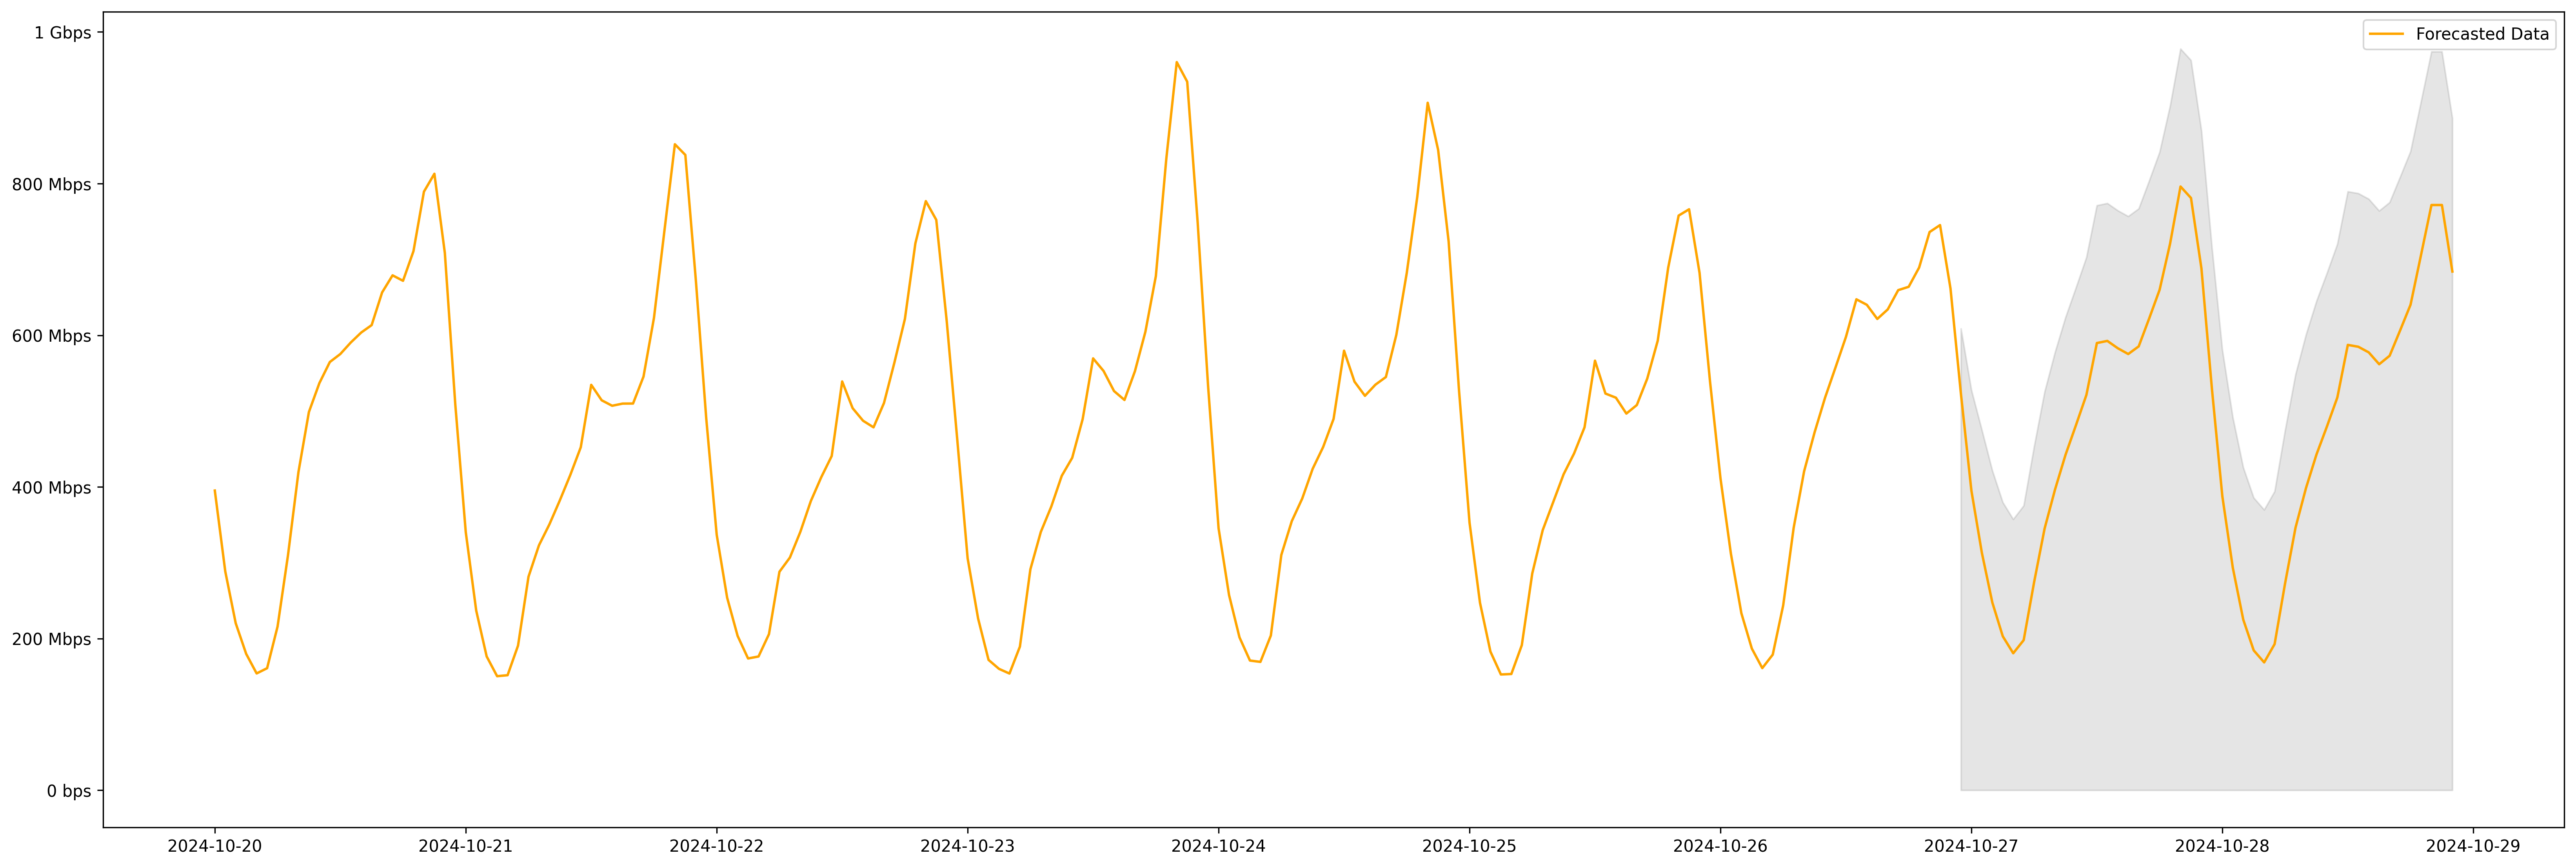
\includegraphics[width=.3\textwidth]{paper/images/first-forecasting-sarimax.png}
    }\hfill
    \subfigure[\label{fig:prophet}Prophet]{
        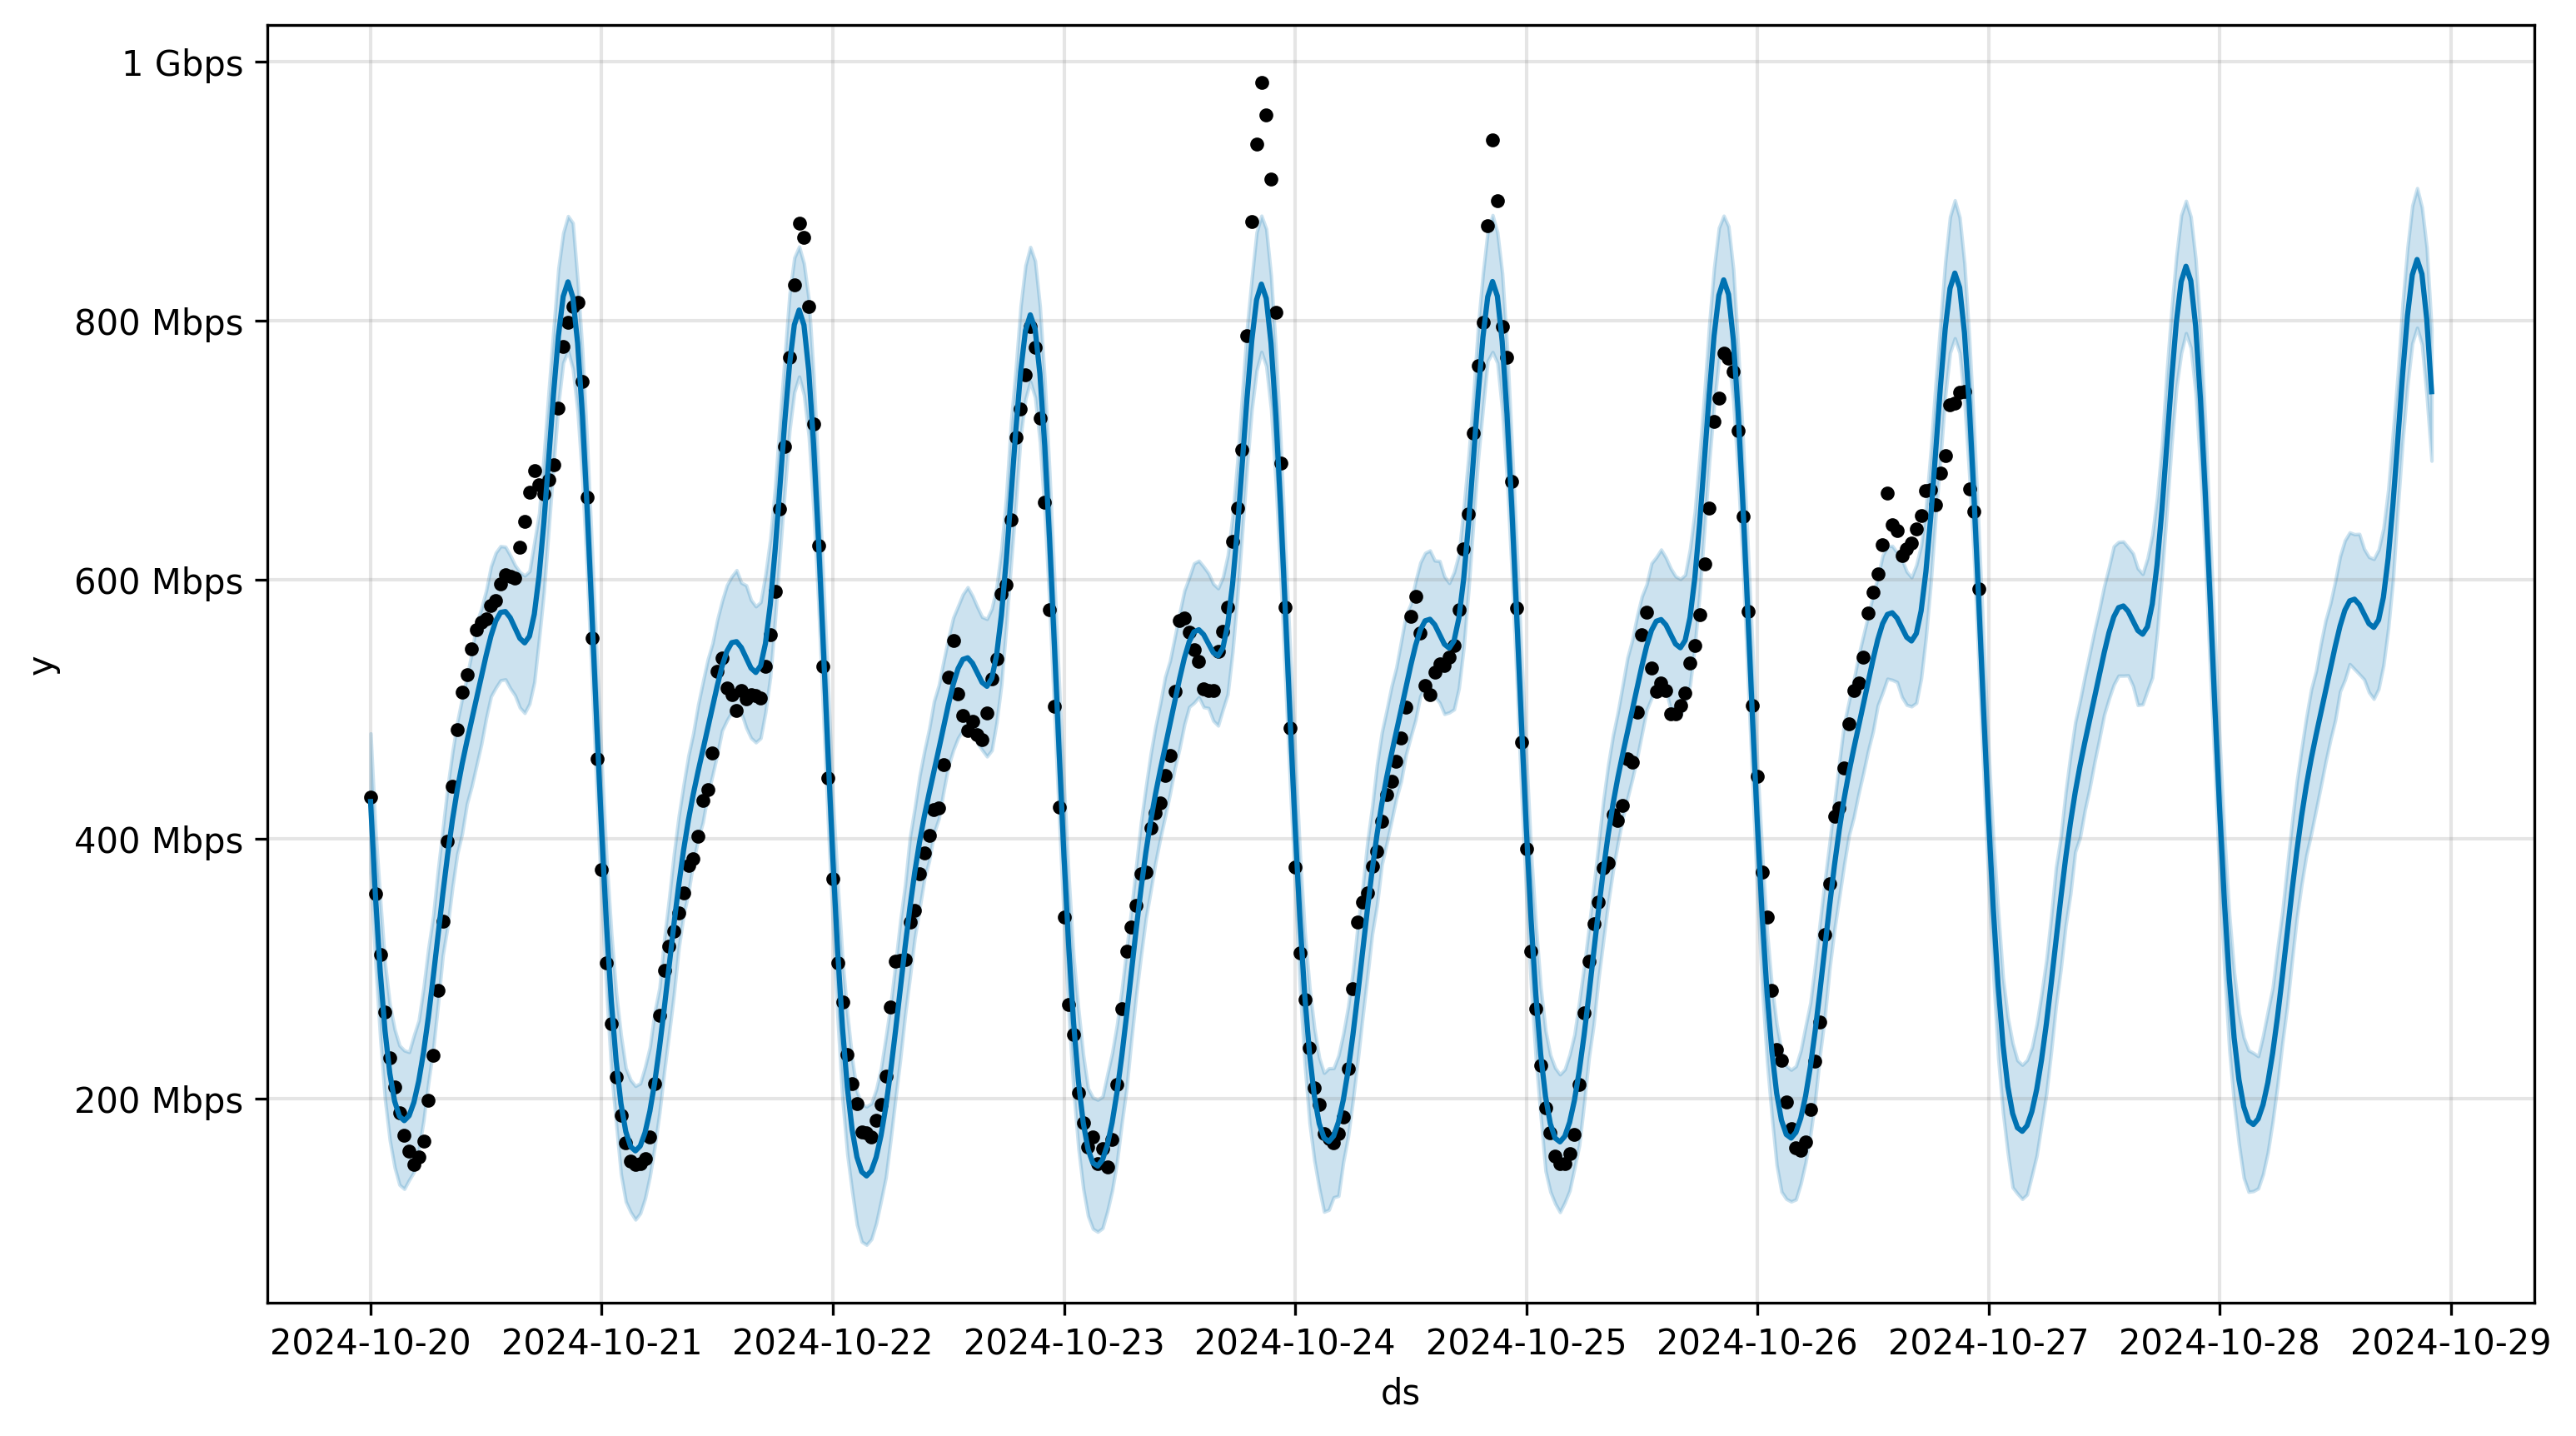
\includegraphics[width=.3\textwidth]{paper/images/first-forecasting-prophet.png}
    }
    \subfigure[\label{fig:lstm}LSTM]{
        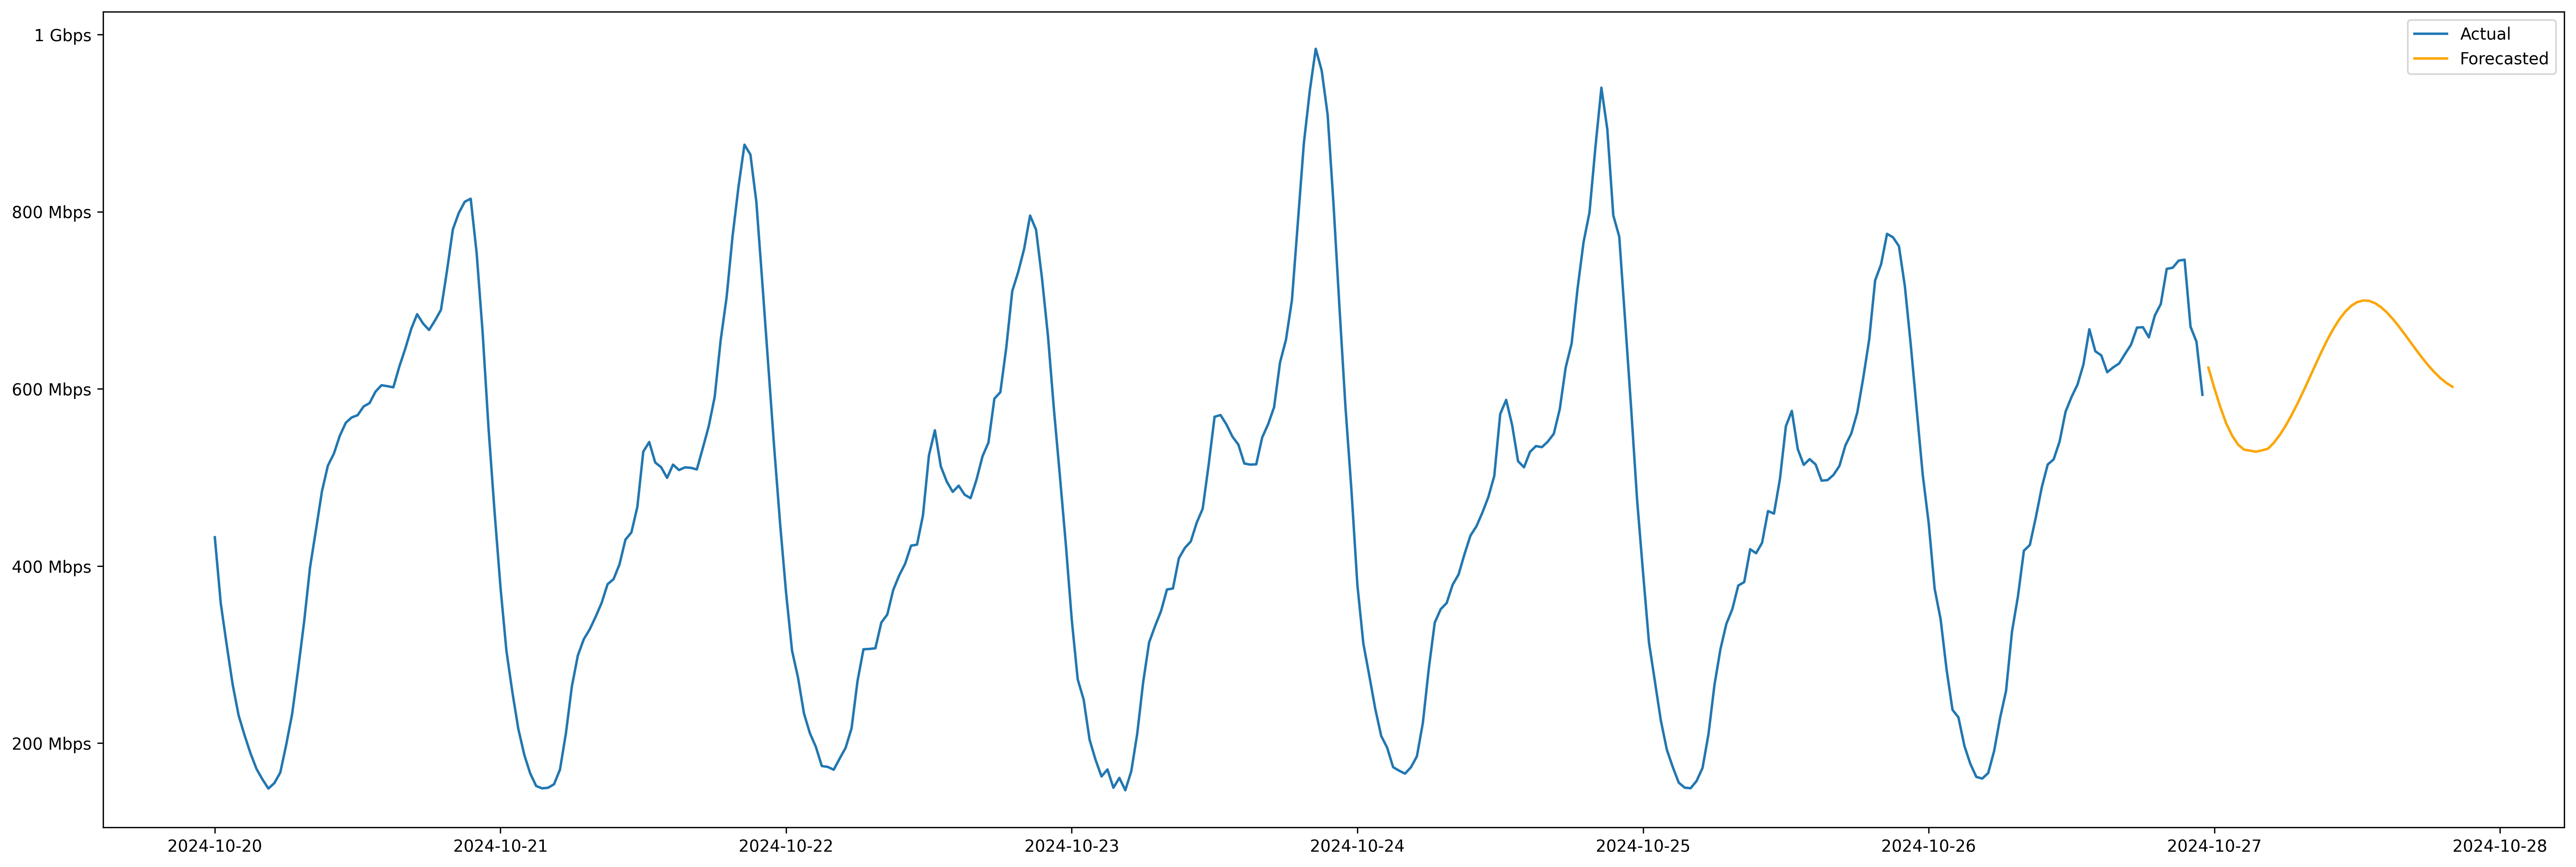
\includegraphics[width=.3\textwidth]{paper/images/first-forecasting-lstm.png}
    }
    \caption{Comparação das previsões utilizando os três modelos}
\end{figure}

\section{Resultados obtidos}

Os melhores resultados de previsão obtidos foram dos modelos estatísticos, tendo em vista que o LSTM não conseguiu prever muito bem o padrão da série temporal, isso em todos os datasets que testamos. Já sob os recursos computacionais, observamos que o Prophet foi o mais "leve" em relação à tempo de treinamento e peso do modelo salvo em armazenamento secundário.

\begin{table}[ht]
\centering
\caption{Comparação do Modelos}
\label{tab:comparing}
\begin{tabular}{lcc}
\toprule
\textbf{Modelo} & \textbf{Tempo de Treinamento} & \textbf{Peso em Disco} \\
\midrule
LSTM     & $\sim$17 segundos & 11 MB \\
SARIMAX & $\sim$4 segundos & 137 MB \\
Prophet  & $\sim$1 segundo   & 140 KB \\
\bottomrule
\end{tabular}
\end{table}

Respondendo às perguntas da seção de Objetivos da Pesquisa, temos os seguintes resultados.

\begin{itemize}
  \item Qual algoritmo estatístico ou de inteligência artificial melhor se adéqua ao cenário do tráfego da minha rede e de meus clientes?
    \SubItem SARIMAX ou Prophet dependendo do objetivo, já que o SARIMAX foi melhor porém mais lento.
  \item Quais são as melhores combinações de hiper-parâmetros para meu tipo de tráfego?
    \SubItem SARIMAX: p3, d0, q1; Prophet: padrão; LSTM: 10 épocas, 96 neuronios, 4 layers.
  \item O tempo para gerar o modelo versus sua eficiência de predição são adequados ao meu caso de uso levando em consideração diferentes vetores da rede?
    \SubItem O Prophet não conseguiu prever os maiores momentos de tráfego, já o SARIMAX sim, então dependendo do contexto podemos empregar um ou o outro.
\end{itemize}

\section{Possíveis melhorias e Trabalhos futuros}

Como podemos observar na seção de avaliaçăo, o modelo LSTM fez uma péssima previsão, porém imaginamos que isso seja por conta da modelagem da rede neural. Em trabalhos futuros, o autor irá desenvolver melhores redes neurais para tentar aumentar os resultados obtidos com o modelo LSTM.

Para trabalhos futuros, o autor estuda formas de correlacionar a previsão do tráfego de rede com novas features de séries temporais também extraídas dos fluxos IP de grandes redes de computadores como ISPs e IXes, com o objetivo de tentar identificar desvios de padrões, tráfego anormal e congestionamento derivado de possíveis ataques com origens globais.

\section{Contexto}

O seguinte trabalho e seus resultados são frutos de um projeto apresentado no final da disciplina da aula de reconhecimento de padrões do curso de Mestrado em Ciência da Computação da Universidade Estadual de Londrina (UEL) e não possui o objetivo de ser publicado como um artigo científico.

\newpage
\printbibliography

\end{document}
